\section{Statistical Analysis of Experiment \#2}\label{sec:Stat2}
In this section the results from experiment \#2 will be analyzed. The expectation from this analysis is to see similar observations to what was found in \cref{sec:Stat1}, possibly with some deviations as a result of the disabled C-State. 

\subsection{Normal distribution}\label{subsec:NormalDist2}

The fist part of the analysis will be the normal distribution for this experiment, analyzed using the Shapiro-Wilk test.

\paragraph{Expectations:} The expectation is to find a similar conclusion as was found when analyzing the first experiment in \cref{sec:Stat1}. In \cref{sec:Stat1} the data was not found to be normally distributed in some cases, but not all.

\begin{table}[]
    \begin{tabular}{||c|c|c|c|c|c||}    \hline
    &\textbf{TestCaseIdle}&\textbf{BinaryTrees}&\textbf{FannkuchRedux}&\textbf{Nbody}&\textbf{Fasta}\\ [0.5ex] \hline
    \hline \textbf{IntelPowerGadget}&0.0&\textbf{0.9103}&\textbf{0.1293}&0.0002&\textbf{0.8291}\\
    \textbf{HardwareMonitor}&0.0213&\textbf{0.1345}&0.0492&\textbf{0.3209}&0.0\\
    \textbf{Clamp Win}&0.0034&0.0023&0.012&\textbf{0.8143}&\textbf{0.5335}\\
    \textbf{RAPL}&\textbf{0.1899}&\textbf{0.5744}&0.0015&\textbf{0.9437}&\textbf{0.0518}\\
    \textbf{Clamp Lin}&\textbf{0.4601}&0.0004&0.0&\textbf{0.1006}&0.0002\\ \hline \end{tabular}
    \caption{P values for the normal distribution for the Workstation in Ex2}\label{tab:NormDist2}
\end{table} 


\paragraph{Results:} The results from the Sharpiro Wilk test can be seen in \cref{tab:NormDist2}. \cref{tab:NormDist2} shows the data is not normally distributed, where the data from this experiment is generally further away from being normally distributed than in \cref{sec:Stat1}. One reason why this experiment is further away from being normally distributed could be a result of fewer measurements compared to the first experiment.

\subsection{Independence Test}\label{subsec:independence2}
It was found in \cref{subsec:NormalDist2}, that the data for this experiment was not normally distributed. Because of this, the Mann Whitney U Test will be used to test independence just like in \cref{subsec:independence1}.

\paragraph{Expectations:} For the MannWhitney U test we would expect very similar results to the results from experiment 1, where the null hypotheses can be rejected in most of the cases. This is because the changes between in experiment 1 and experiment 2 would not change the independence of the data, so should not change the result remarkably

\begin{figure}
    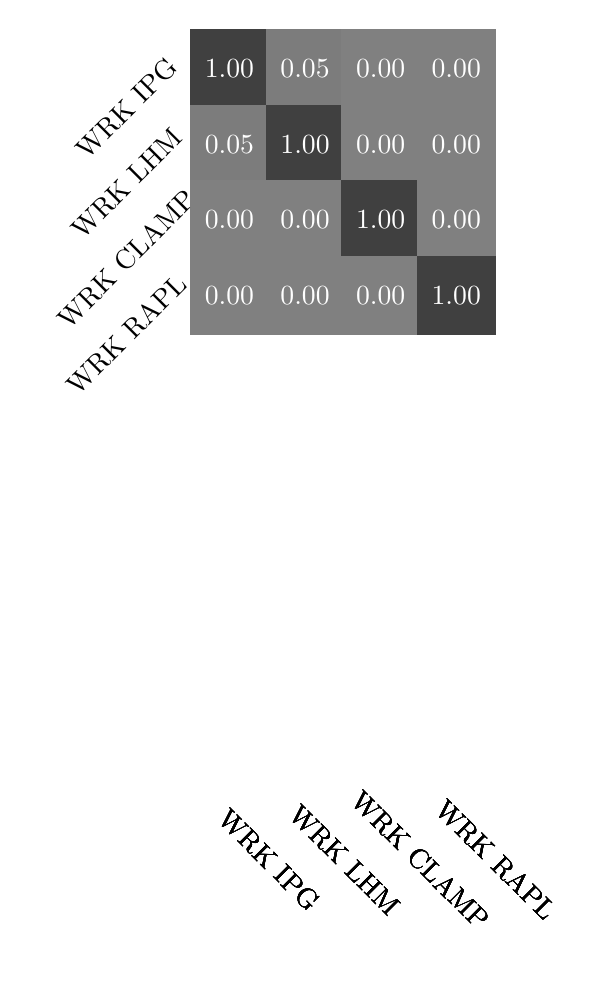
\begin{tikzpicture}[scale=0.6]
      \foreach \y [count=\n] in {{1.00, 0.05, 0.00, 0.00},{0.05, 1.00, 0.00, 0.00},{0.00, 0.00, 1.00, 0.00},{0.00, 0.00, 0.00, 1.00},} {
      % column labels
      \foreach \a [count=\n] in {WRK IPG,WRK LHM,WRK CLAMP,WRK RAPL} {
        \node[minimum size=10mm, xshift=0.5cm, rotate=-45] at (\n*1.6, -18.35) {\a};
      }
      % heatmap tiles
      \foreach \x [count=\m] in \y {
        \pgfmathsetmacro{\xa }{(\x + 1) / 2 * 100}
        \node[fill=darkgray!\xa!lightgray, minimum size=10mm, text=white, font={\normalsize}] at (\m*1.6,-\n*1.6) {\x};
      }
    }
      % row labels
      \foreach \a [count=\i] in {WRK IPG,WRK LHM,WRK CLAMP,WRK RAPL} {
        \node[minimum size=10mm, xshift=-0.35cm, yshift=-0.5cm, rotate=45] at (0,-\i*1.6) {\a};
      }
    \end{tikzpicture}
    \label{tab:HeatFannkuchRedux2}
\end{figure}

\paragraph{Results:} The results from the MannWhitney U test can be seen here in \cref{tab:HeatFannkuchRedux2}, where the results from the rest of the test cases can be found in \cref{app:stat2}. The shown table in \cref{tab:HeatFannkuchRedux2} the results from the test case FannkuchRedux can be seen, where a similar tendency to the first experiment can be seen. This tendency being that we can reject $H_0$ in most cases. When comparing this analysis the one conducted on the first experiment, we find more cases where we cannot reject $H_0$ in this experiment. This could be a result of less measurements compared to the first experiment, meaning outliers has a larger effect.

\subsection{Correlation}\label{subsec:correlation2}
In this section the correlation between the different measurement instrument will be conducted for the second experiment. The Kendall Tau correlation coefficients will again be used as it was in \cref{subsec:correlation1}

\paragraph{Expectations:} The expectations for the correlations when the C-states are disabled will either be a similar or higher correlation. If the similarity increases, it would be expected to be because the uncertainty of the C-states has been removed.

\begin{figure}
    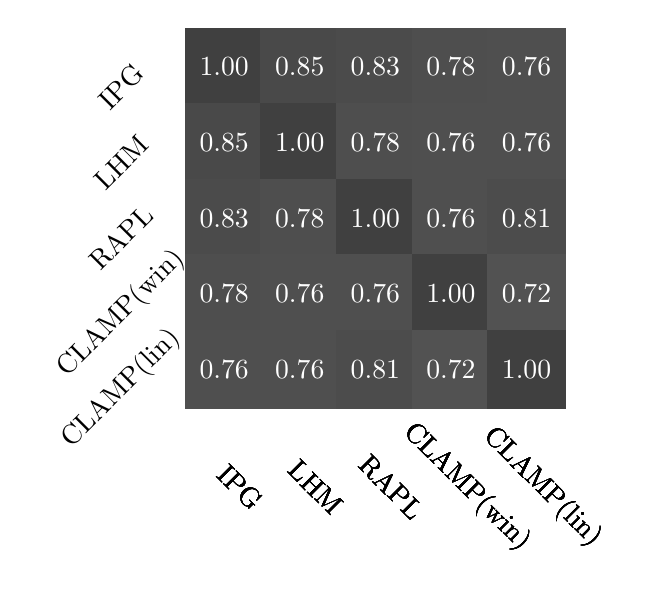
\begin{tikzpicture}[scale=0.6]
      \foreach \y [count=\n] in {{1.00, 0.85, 0.83, 0.78, 0.76},{0.85, 1.00, 0.78, 0.76, 0.76},{0.83, 0.78, 1.00, 0.76, 0.81},{0.78, 0.76, 0.76, 1.00, 0.72},{0.76, 0.76, 0.81, 0.72, 1.00},} {
      % column labels
      \foreach \a [count=\n] in {IPG,LHM,RAPL,CLAMP(win),CLAMP(lin)} {
        \node[minimum size=10mm, xshift=0.2cm, rotate=-45] at (\n*1.6, -10.5) {\a};
      }
      % heatmap tiles
      \foreach \x [count=\m] in \y {
        \pgfmathsetmacro{\xa }{(\x + 1) / 2 * 100}
        \node[fill=darkgray!\xa!lightgray, minimum size=10mm, text=white, font={\normalsize}] at (\m*1.6,-\n*1.6) {\x};
      }
    }
      % row labels
      \foreach \a [count=\i] in {IPG,LHM,RAPL,CLAMP(win),CLAMP(lin)} {
        \node[minimum size=10mm, xshift=-0.35cm, yshift=-0.25cm, rotate=45] at (0,-\i*1.6) {\a};
      }
    \end{tikzpicture}
    \label{tab:correlationWork2}
\end{figure}

\paragraph{Results:} The calculated Correlations for this experiment can be seen in \cref{tab:correlationWork2}. These results look very similar to the similarities obtained from the first experiment in \cref{subsec:correlation1}. The average correlation from experiments on the workstation are as following:

$$\text{AvgCoefEx1} = (0.81+0.80+0.77+0.71+0.80+0.78+0.71+0.77+0.72+0.70)/10 = 0.757$$
$$\text{AvgCoefEx2} = (0.85+0.83+0.78+0.76+0.78+0.76+0.76+0.76+0.81+0.72)/10 = 0.781$$

These coefficients show a higher correlations between the different DUTs and their measurement instruments. Next up, the coefficients will be analyzed and utilized to answer our research questions. 

\paragraph{RQ2:} When comparing the measurement instruments to each other the average correlation foreach instrument can be calculated. These will then be compared with the results from \cref{sec:Stat1}, to see what effect disabling the C-States have had on the measurements.

\begin{itemize}
    \item \textbf{Experiment 1}
    \begin{itemize}
        \item $IPG = 0.772$ %0.81+0.80+0.77+0.71
        \item $LHM = 0.775$ %0.81+0.80+0.78+0.71
        \item $RAPL = 0.725$ %0.80+0.80+0.77+0.72
        \item $CLAMP(win) = 0.755$ %0.77+0.78+0.77+0.70
        \item $CLAMP(lin) = 0.710$ %0.71+0.71+0.72+0.70
    \end{itemize}
    \item \textbf{Experiment 2}
    \begin{itemize}
        \item $IPG = 0.805$ %0.85+0.83+0.78+0.76
        \item $LHM = 0.787$ %0.85+0.78+0.76+0.76
        \item $RAPL = 0.795$%0.83+0.78+0.76+0.81
        \item $CLAMP(win) = 0.755$ %0.78+0.76+0.76+0.72
        \item $CLAMP(lin) = 762$ % 0.76+0.76+0.81+0.72
    \end{itemize}
\end{itemize}

When looking at the average correlation for the measurement instruments across the two experiments, the second experiment generally had larger coefficients than the first experiment, showing a higher correlation for the second experiment. Looking at these number using the Guildford scale, it can be seen how the correlation does not increase enought to change evaluation, as we expected.

\paragraph{RQ3:} When comparing the results across OSs, some differences can be observed when compared with the first experiment. The OS benefitting the most in terms of correlation coefficients when disabling the C-Stats is linux, as the correlation between RAPL and the other measuring instruments increased. This is mostly dues to an increased correlation between RAPL and the clamp on Linux, which increased from $0.72$ to $0.81$.  Overall it seems that RAPL is the measuring instrument most closely correlated with the hardware measurements while IPG is the most correlated measuring instrument for Windows.





% \begin{table}[]
    \begin{tabular}{||c|c|c|c|c|c||}    \hline
    &\textbf{TestCaseIdle}&\textbf{BinaryTrees}&\textbf{FannkuchRedux}&\textbf{Nbody}&\textbf{Fasta}\\ [0.5ex] \hline
    \hline \textbf{IntelPowerGadget}&0.0&\textbf{0.9103}&\textbf{0.1293}&0.0002&\textbf{0.8291}\\
    \textbf{HardwareMonitor}&0.0213&\textbf{0.1345}&0.0492&\textbf{0.3209}&0.0\\
    \textbf{Clamp Win}&0.0034&0.0023&0.012&\textbf{0.8143}&\textbf{0.5335}\\
    \textbf{RAPL}&\textbf{0.1899}&\textbf{0.5744}&0.0015&\textbf{0.9437}&\textbf{0.0518}\\
    \textbf{Clamp Lin}&\textbf{0.4601}&0.0004&0.0&\textbf{0.1006}&0.0002\\ \hline \end{tabular}
    \caption{P values for the normal distribution for the Workstation in Ex2}\label{tab:NormDist2}
\end{table} 

% As can be seen in \cref{tab:NormDist2}, the data is not normally distributed the data from experiment 2 is generally further away from being normally distributed than the experiment 1. This is not that surprising given that experiment 2 contain less actual runs as these were not needed as found in \cref{subsec:CockUse}. 

% For the MannWhitney U test we would again expect very similar results to the results from experiment one, where the null hypotheses can be rejected in most of the cases.
% The results from the MannWhitney U test can be seen here in \cref{tab:HeatFannkuchRedux2}.
% \begin{figure}
    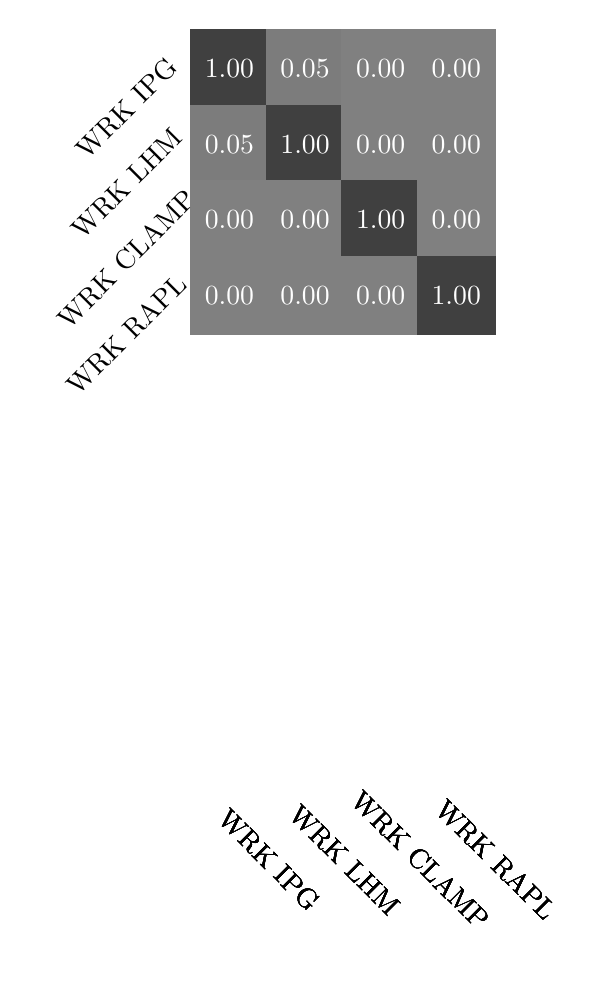
\begin{tikzpicture}[scale=0.6]
      \foreach \y [count=\n] in {{1.00, 0.05, 0.00, 0.00},{0.05, 1.00, 0.00, 0.00},{0.00, 0.00, 1.00, 0.00},{0.00, 0.00, 0.00, 1.00},} {
      % column labels
      \foreach \a [count=\n] in {WRK IPG,WRK LHM,WRK CLAMP,WRK RAPL} {
        \node[minimum size=10mm, xshift=0.5cm, rotate=-45] at (\n*1.6, -18.35) {\a};
      }
      % heatmap tiles
      \foreach \x [count=\m] in \y {
        \pgfmathsetmacro{\xa }{(\x + 1) / 2 * 100}
        \node[fill=darkgray!\xa!lightgray, minimum size=10mm, text=white, font={\normalsize}] at (\m*1.6,-\n*1.6) {\x};
      }
    }
      % row labels
      \foreach \a [count=\i] in {WRK IPG,WRK LHM,WRK CLAMP,WRK RAPL} {
        \node[minimum size=10mm, xshift=-0.35cm, yshift=-0.5cm, rotate=45] at (0,-\i*1.6) {\a};
      }
    \end{tikzpicture}
    \label{tab:HeatFannkuchRedux2}
\end{figure}
% The shown table in \cref{tab:HeatFannkuchRedux2}, is again from the FannkuchRedux Test Case as in \cref{subsec:Stat1}. Again we see a similar tendency in that for most cases we can reject $H_0$, but for experiment 2 there are a few more cases where we cannot reject $H_0$. Once possible reason why that might be the case is that there are fewer samples in experiment 2 so outlier have a larger effect on the Ex1Statistics.

% Finally for the Correlations between the measuring instruments, the expectations for the correlations in Experiment 2 is that they are either are a bit more correlated since the uncertainty's of the C-Stats have been removed, or that i will remain nearly exactly the same. The calculated Correlations for experiments 2 can be seen in \cref{tab:correlationWork2}.
% \begin{figure}
    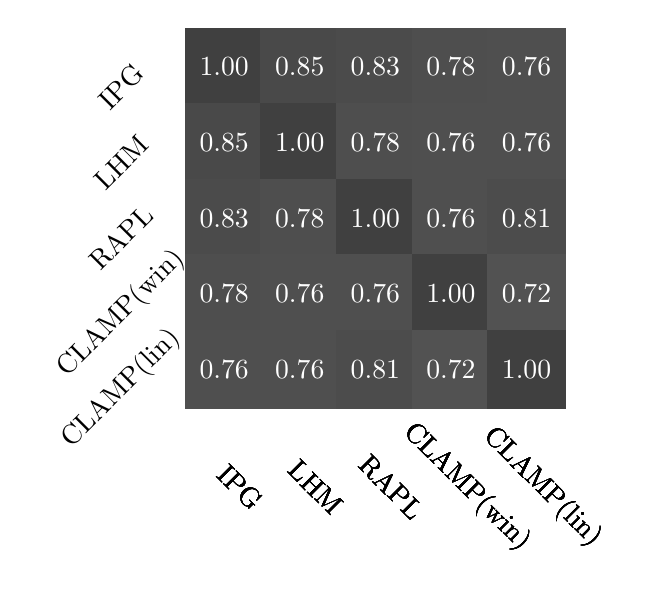
\begin{tikzpicture}[scale=0.6]
      \foreach \y [count=\n] in {{1.00, 0.85, 0.83, 0.78, 0.76},{0.85, 1.00, 0.78, 0.76, 0.76},{0.83, 0.78, 1.00, 0.76, 0.81},{0.78, 0.76, 0.76, 1.00, 0.72},{0.76, 0.76, 0.81, 0.72, 1.00},} {
      % column labels
      \foreach \a [count=\n] in {IPG,LHM,RAPL,CLAMP(win),CLAMP(lin)} {
        \node[minimum size=10mm, xshift=0.2cm, rotate=-45] at (\n*1.6, -10.5) {\a};
      }
      % heatmap tiles
      \foreach \x [count=\m] in \y {
        \pgfmathsetmacro{\xa }{(\x + 1) / 2 * 100}
        \node[fill=darkgray!\xa!lightgray, minimum size=10mm, text=white, font={\normalsize}] at (\m*1.6,-\n*1.6) {\x};
      }
    }
      % row labels
      \foreach \a [count=\i] in {IPG,LHM,RAPL,CLAMP(win),CLAMP(lin)} {
        \node[minimum size=10mm, xshift=-0.35cm, yshift=-0.25cm, rotate=45] at (0,-\i*1.6) {\a};
      }
    \end{tikzpicture}
    \label{tab:correlationWork2}
\end{figure}
% At an first these results look very similar to the once from experiment 1, but to verify these number more in depth we can compare the averages of the correlations as before.


% This slight increase in overall correlation matches up with our expectations as the added consistency in the experiments should help reduce inconsistencies. Generally the correlations are higher in experiment 2, but the correlation does fall in certain cases, these cases will be looked at a bit here.

% The first case is the $RAPL|CLAMP(win)$ which used to in experiment one to have a coefficients of $0.77$, but in Experiment 2 as $0.76$, while this is only a marginal decrease it could be caused by the fact that one measures linux and the other windows. Another one is $LHM|RAPL$ which went from $0.80$ to $0.78$ these measurements are again done on separate OSs. 

% So the divide between linux and windows seems to have gotten larger.   









